\documentclass[12pt]{article}
\usepackage[english]{babel}
\usepackage{float}
\usepackage[margin=1in]{geometry}
\usepackage{graphicx}
%\usepackage[toc,page]{appendix}
\graphicspath{ {./doc/img/} }
\newcommand{\rpm}{\raisebox{.2ex}{$\scriptstyle\pm$}} 
\usepackage{listings}
\usepackage{xcolor}
\usepackage{indentfirst}
\usepackage[final]{pdfpages}


\begin{document}

\title{Joe Phaneuf \\ Computer Vision 16-720 Spring 2018 \\ Feb. 03, 2018 }
\date{}
\author{}
\maketitle

\newpage


%\stepcounter{section}
%%%%%%%%%%%%%%%%%%%%%%%%%%%%%%%%%%%%%%%%%%%%%%%%%%%%%%%%%%%%%%%%%%%%%%%%%%%%%%%%
%%%%%%%%%%%%%%%%%%%%%%%%%%%%%%%%%%%%%%%%%%%%%%%%%%%%%%%%%%%%%%%%%%%%%%%%%%%%%%%%
\section{Q1}
\subsection{Q1.1}

The filter bank contains four types of filters at different scales. The first two filters (gaussian and log) will respond to circular elements, the former containing peaks and the latter containing valleys.
The next two filter types are derivitive filters, which will respond to vertical and horizontal edges respectively.
Figure \ref{fig:test_image} shows a test image for the filters, Figure shows \ref{fig:filters} the filters themselves, while Figure \ref{fig:filter_responses} shows the filtered images.

\begin{figure}[H]
\centering
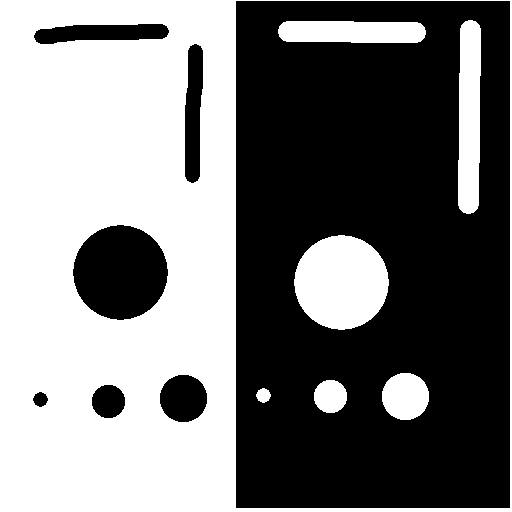
\includegraphics[page=1,width=0.4\textwidth]{test}
\caption{Test image}    
\label{fig:test_image}
\end{figure}   

\begin{figure}[H]
\centering
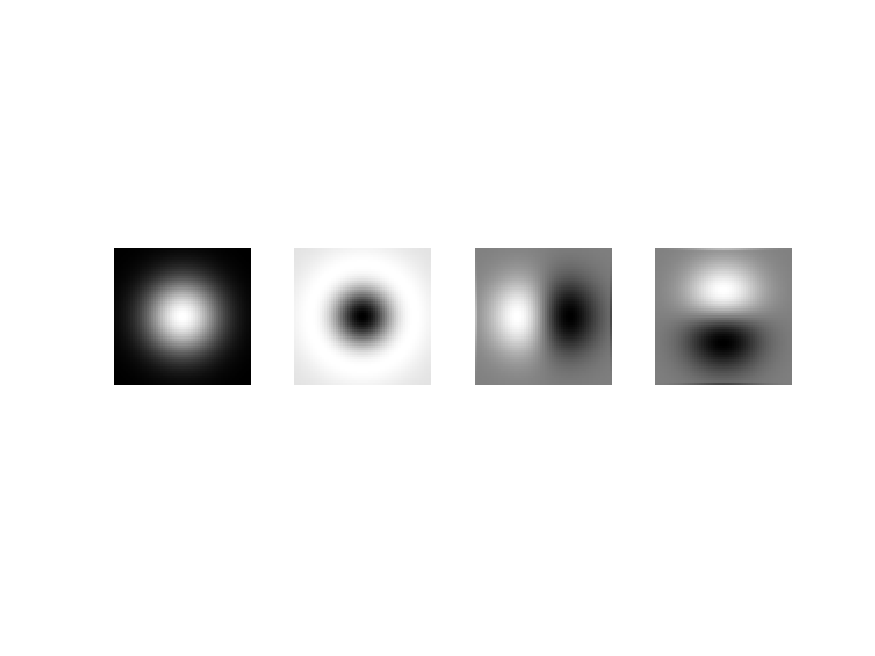
\includegraphics[page=1,width=0.75\textwidth]{q1_filters}
\caption{Filters}    
\label{fig:filters}
\end{figure}   

\begin{figure}[H]
\centering
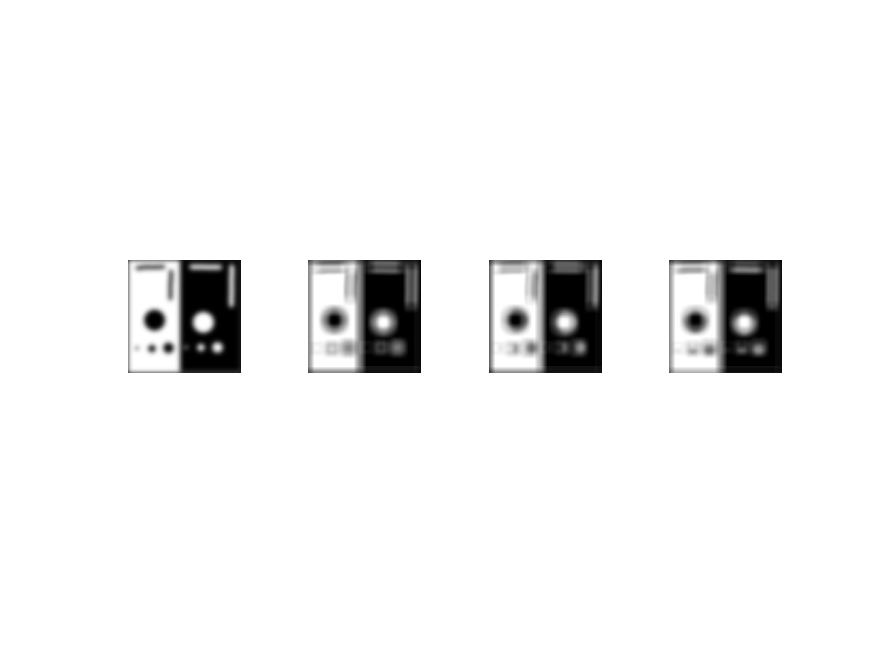
\includegraphics[page=1,width=0.75\textwidth]{q1_responses}
\caption{Filter responses}    
\label{fig:filter_responses}
\end{figure}   

%%%%%%%%%%%%%%%%%%%%%%%%%%%%%%%%%%%%%%%%%%%%%%%%%%%%%%%%%%%%%%%%%%%%%%%%%%%%%%%%
%%%%%%%%%%%%%%%%%%%%%%%%%%%%%%%%%%%%%%%%%%%%%%%%%%%%%%%%%%%%%%%%%%%%%%%%%%%%%%%%
\newpage
\subsection{Q1.2}
The extractFilterResponses function convertes an input image to the CIE LAB color space, and subsequently applies the filter bank described above to each channel (L A B).
The CIE LAB color space is chosen for this application as the image intensity is stored in a separate channel (L) from color information (A B). In RGB colorspace (default for most input images), image intensity is a combination of all channels, and image processing techniques are therefore highly sensitive to the lighting conditions in which the image was captured. The CIE LAB color space color channels will be more similar for images of the same object in different lighting conditions. Figure \ref{fig:extract_filter_responses} shows a sample image along with one feature filter applied to the L, A, and B channels.

\begin{figure}[H]
\centering
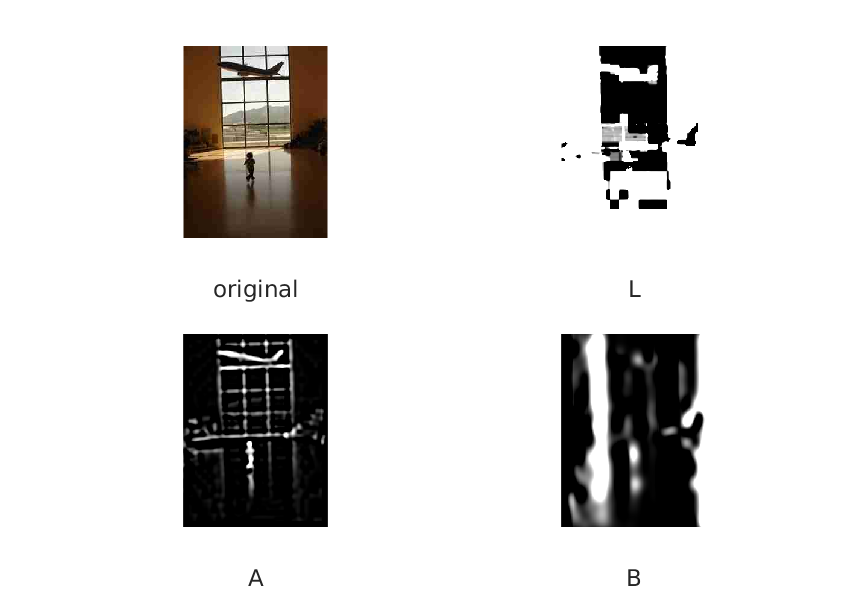
\includegraphics[page=1,width=0.75\textwidth]{q12_extract_filters}
\caption{Filter responses on LAB colored images}    
\label{fig:extract_filter_responses}
\end{figure}   

%%%%%%%%%%%%%%%%%%%%%%%%%%%%%%%%%%%%%%%%%%%%%%%%%%%%%%%%%%%%%%%%%%%%%%%%%%%%%%%%
%%%%%%%%%%%%%%%%%%%%%%%%%%%%%%%%%%%%%%%%%%%%%%%%%%%%%%%%%%%%%%%%%%%%%%%%%%%%%%%%
\newpage
\subsection{Q1.3}

Figure \ref{fig:harris_corners} shows my Harris corner detector applied to three images.

\begin{figure}[H]
\centering
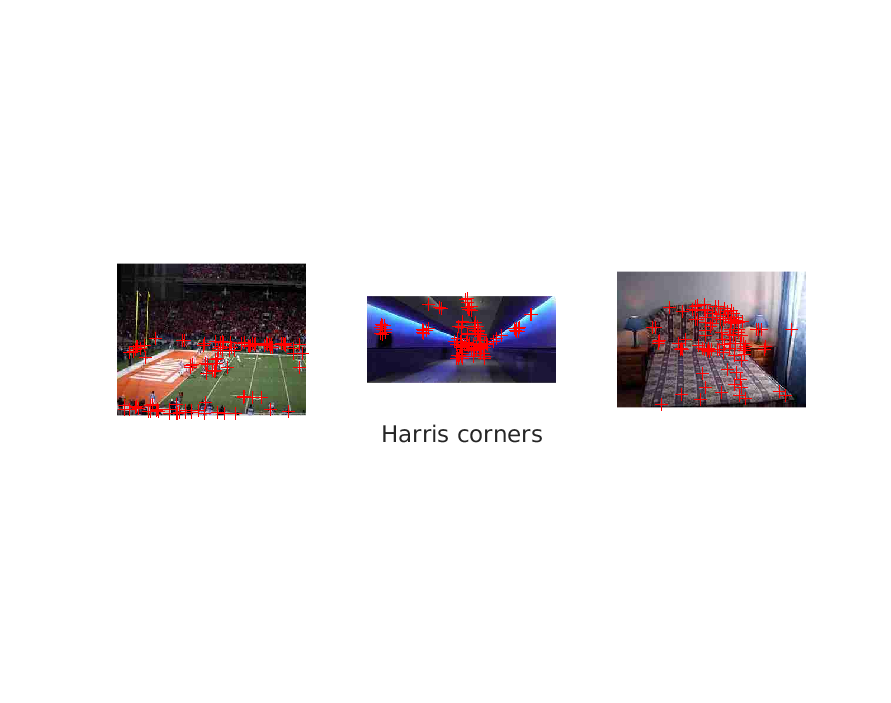
\includegraphics[page=1,width=1\textwidth]{q13_harris}
\caption{Harris corners}    
\label{fig:harris_corners}
\end{figure}   

%%%%%%%%%%%%%%%%%%%%%%%%%%%%%%%%%%%%%%%%%%%%%%%%%%%%%%%%%%%%%%%%%%%%%%%%%%%%%%%%
%%%%%%%%%%%%%%%%%%%%%%%%%%%%%%%%%%%%%%%%%%%%%%%%%%%%%%%%%%%%%%%%%%%%%%%%%%%%%%%%
\newpage
\section{Q2}
\subsection{Q2.1}

Figure \ref{fig:wordmapharris} shows the word map produced on 3 images of airport and rainforest class using the harris corner generated dictionary.
Figure \ref{fig:wordmaprandom} shows the word map produced on 3 images of airport and rainforest class using the random corner generated dictionary.
The goal of viewing these images is to capture semantic labeling on swatchs of an image, so "better" means more contiguous space logically grouped together (i.e. all pixels of a swath of grass have the same label.) The word maps from the harris dictionary appear to accomplish this better than the word maps from the random dictionary.

\begin{figure}[H]
\centering
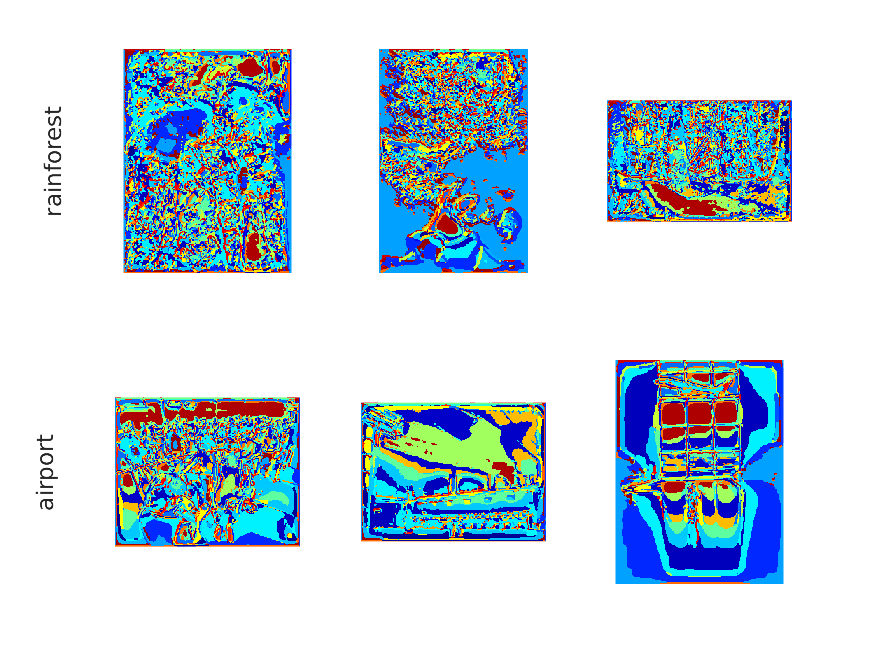
\includegraphics[page=1,width=1\textwidth]{q21_wordmap_harris}
\caption{Wordmap Harris corners corners}    
\label{fig:wordmapharris}
\end{figure}   


\begin{figure}[H]
\centering
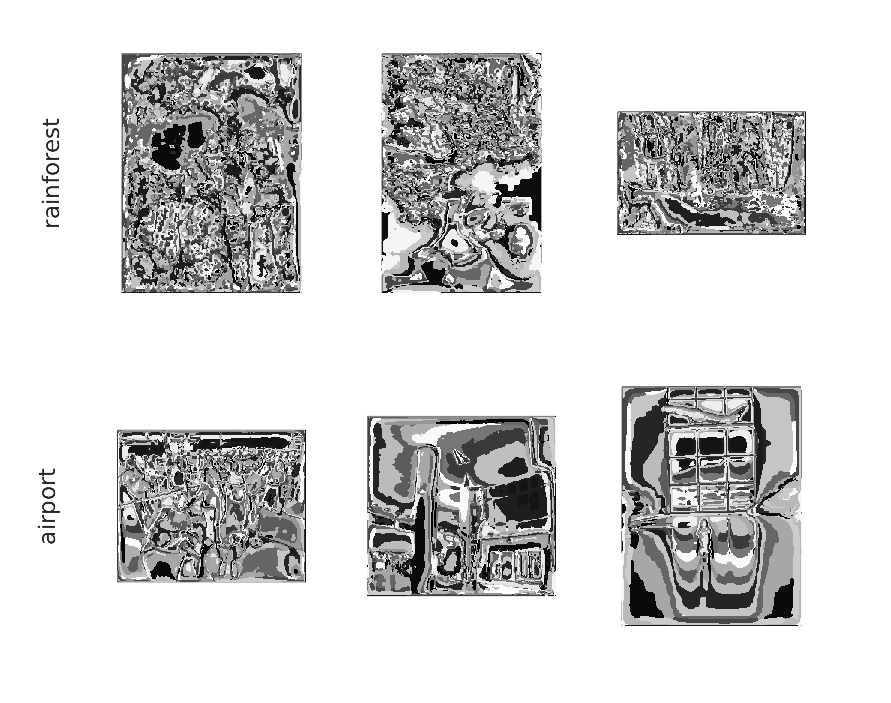
\includegraphics[page=1,width=1\textwidth]{q21_wordmap_random}
\caption{Wordmap random corners}    
\label{fig:wordmaprandom}
\end{figure}   

%%%%%%%%%%%%%%%%%%%%%%%%%%%%%%%%%%%%%%%%%%%%%%%%%%%%%%%%%%%%%%%%%%%%%%%%%%%%%%%%
%%%%%%%%%%%%%%%%%%%%%%%%%%%%%%%%%%%%%%%%%%%%%%%%%%%%%%%%%%%%%%%%%%%%%%%%%%%%%%%%
\newpage
\section{Q3}
\subsection{Q3.2}

The tables below show visual bag of words accuracies and confusion matrices for the permutations of harris corner / random point and euclidean / chi2 distance.  Harris corners outperform random points , and the chi2 distance outperforms euclidean distance, with the overall winner being harris corners + chi2 distance. This tracks with the notion the harris corners should identify more useful features to train on than randomly selecting points. This also makes sense as chi2 distance is more of a measure of simalarity than a 'spatial' euclidean distance.


\subsubsection{confusion matrix harris chi2}


     6     1     4     1     0     0     3     5
     5     8     4     2     0     0     0     1
     1     0    12     2     1     0     2     2
     2     3     2     8     0     0     2     3
     0     2     5     0     7     0     6     0
     4     1     1     0     2     7     3     2
     2     1     6     4     1     0     6     0
     0     1     0     2     0     0     0    17


accuracy = 0.4437


\subsubsection{confusion matrix harris euclidean}

     5     2     3     3     0     1     1     5
     2     9     3     1     0     1     0     4
     2     1    10     2     0     0     4     1
     4     6     1     2     0     1     4     2
     3     1     2     2     5     0     5     2
     4     3     4     2     3     2     0     2
     1     6     4     2     1     1     3     2
     0     1     0     5     0     0     0    14

accuracy = 
    0.3125

\subsubsection{confusion matrix random chi2}

     8     0     3     3     0     1     1     4
     3     5     2     1     0     1     4     4
     4     1    10     2     2     0     1     0
     4     4     0     5     1     0     4     2
     0     2     4     1     7     0     6     0
     2     0     1     1     3     6     2     5
     3     0     5     2     2     1     4     3
     0     1     0     1     0     0     0    18


accuracy = 0.3937

\subsubsection{confusion matrix random euclidean}


     5     0     4     2     1     1     2     5
     7     3     2     1     0     0     2     5
     4     0     9     2     3     0     1     1
     3     4     2     4     1     0     3     3
     1     1     6     0     4     0     6     2
     5     1     3     2     1     4     2     2
     1     8     4     1     1     1     1     3
     1     2     0     3     0     1     0    13


accuracy = 0.2687

\end{document}
